\documentclass{beamer}                             % presentation
% \documentclass[draft]{beamer}                    % improves compile time
% 4' x 3' poster (48" x 36")
\usepackage[orientation=landscape,size=custom,width=121.92,height=91.44,
scale=1.4,debug]{beamerposter}
% replace default beamer blocks for more customization of outlines
% https://tex.stackexchange.com/questions/11484/how-to-draw-a-frame-box-around-an-arbitrary-large-piece-of-text-figures-whatever
\usepackage{tcolorbox}
\usepackage[utf8]{inputenc}                        % utf8
\usepackage[T1]{fontenc}                           % fix font encoding
\usepackage{lmodern}                               % arbitrarily large font
\usepackage[english]{babel}                        % language
\usepackage{geometry, hyperref, fancyhdr, algorithm}
\usepackage{amsmath, amssymb, amsthm}              % ams mathematical packages
\usepackage{physics, mathtools, bm}                % extra math packages
\usepackage{graphicx, subcaption, wrapfig}         % images
\usepackage{svg}                                   % svg images
\usepackage{fvextra, textcomp, CJKutf8}            % misc. text formatting
\usepackage[autostyle, english=american]{csquotes} % quotes
\usepackage{tikz, pgfplots}                        % plots and graphs
\usepackage[noend]{algpseudocode}                  % algorithm psuedocode
\usepackage[cache=true]{minted}                    % source code
\usepackage[style=ieee]{biblatex}                  % bibliography

\usetikzlibrary{positioning}                       % advanced positioning
\pgfplotsset{compat=newest}                        % version of pgfplots

\graphicspath{{./figures/}}
\addbibresource{cholesky.bib}

\newcommand{\blocktitle}[1]{{\Large \textbf{#1}}}

% serif font in math mode
% https://ctan.math.utah.edu/ctan/tex-archive/fonts/lm/tex/latex/lm/lmodern.sty
% \usefonttheme[onlymath]{serif}
\renewcommand\mathfamilydefault{cmr}

\SetSymbolFont{operators}   {normal}{OT1}{cmr} {m}{n}
\SetSymbolFont{letters}     {normal}{OML}{cmm} {m}{it}
\SetSymbolFont{symbols}     {normal}{OMS}{cmsy}{m}{n}
\SetSymbolFont{largesymbols}{normal}{OMX}{cmex}{m}{n}
\SetSymbolFont{operators}   {bold}  {OT1}{cmr} {bx}{n}
\SetSymbolFont{letters}     {bold}  {OML}{cmm} {b}{it}
\SetSymbolFont{symbols}     {bold}  {OMS}{cmsy}{b}{n}
\SetSymbolFont{largesymbols}{bold}  {OMX}{cmex}{m}{n}

\SetMathAlphabet{\mathbf}{normal}{OT1}{cmr}{bx}{n}
\SetMathAlphabet{\mathsf}{normal}{OT1}{cmss}{m}{n}
\SetMathAlphabet{\mathit}{normal}{OT1}{cmr}{m}{it}
\SetMathAlphabet{\mathtt}{normal}{OT1}{cmtt}{m}{n}
\SetMathAlphabet{\mathbf}{bold}  {OT1}{cmr}{bx}{n}
\SetMathAlphabet{\mathsf}{bold}  {OT1}{cmss}{bx}{n}
\SetMathAlphabet{\mathit}{bold}  {OT1}{cmr}{bx}{it}
\SetMathAlphabet{\mathtt}{bold}  {OT1}{cmtt}{m}{n}

\renewcommand{\vec}[1]{\bm{#1}}

\DeclareMathOperator{\logdet}{logdet}
\DeclareMathOperator{\chol}{chol}

\DeclareMathOperator*{\argmax}{argmax}
\DeclareMathOperator*{\argmin}{argmin}

\DeclareMathOperator{\E}{E}
\DeclareMathOperator{\Var}{Var}
\DeclareMathOperator{\Cov}{Cov}
\DeclareMathOperator{\info}{I}
\DeclareMathOperator{\entropy}{H}

%%% colors

\definecolor{lightblue}{HTML}{a1b4c7}
\definecolor{orange}{HTML}{ea8810}
\definecolor{silver}{HTML}{b0aba8}
\definecolor{rust}{HTML}{b8420f}
\definecolor{seagreen}{HTML}{23553c}

\colorlet{lightsilver}{silver!20!white}
\colorlet{darkorange}{orange!85!black}
\colorlet{darksilver}{silver!85!black}
\colorlet{darklightblue}{lightblue!75!black}
\colorlet{darkrust}{rust!85!black}
\colorlet{darkseagreen}{seagreen!85!black}

\hypersetup{
  colorlinks=true,
  linkcolor=darkrust,
  citecolor=darkseagreen,
  urlcolor=darksilver
}

%%% beamer settings

\usetheme{Pittsburgh}

% hide navigation buttons
\setbeamertemplate{navigation symbols}{}
% change title color
\setbeamercolor{title}{fg=darklightblue}
\setbeamercolor{frametitle}{fg=darklightblue}
% change bibliography entry colors
\setbeamercolor{bibliography entry author}{fg=darklightblue}
\setbeamercolor{bibliography entry note}{fg=lightblue}

% blocks - use tcolorbox instead of beamer blocks
% \setbeamercolor{block title}{fg=black}
% \setbeamercolor{block body}{bg=lightblue}

% https://mirrors.concertpass.com/tex-archive/macros/latex/contrib/tcolorbox/tcolorbox.pdf
\tcbset{colframe=darklightblue, colback=white}

% margin
\setbeamersize{text margin left=1.27cm, text margin right=1.27cm}

% title page
\title[]{\Huge Sparse Cholesky Factorization by \\
Greedy Conditional Selection}
\subtitle{}
\author[Huan]{\LARGE Stephen Huan and Florian Sch{\"a}fer}
% \institute[Georgia Institute of Technology]
% {
%   Georgia Institute of Technology
% }
\date[]{}
\subject{Computer Science}

\begin{document}
% top align frame
% https://tex.stackexchange.com/questions/16447/beamer-top-aligning-columns-within-a-top-aligned-frame
\begin{frame}[t]
\titlepage

% GT logo in top left
\begin{tikzpicture}[overlay,remember picture]
  \node[below right=4cm and 1.27cm] at (current page.north west) {
      \includesvg[width=0.25\columnwidth]{GTLogoSeal_RGB}
  };
\end{tikzpicture}

% QR code in top right
\begin{tikzpicture}[overlay,remember picture]
  \node[below left=1.27cm and 1.27cm] at (current page.north east) {
      \includesvg[width=0.1\columnwidth]{qrcode}
    };
\end{tikzpicture}

% remove gap
\vspace{-8cm}

\begin{center}
  \textcolor{darksilver}{\rule{\textwidth}{2mm}}
\end{center}

\begin{columns}[T]

%%% column 1

\begin{column}{0.30\textwidth}
  \begin{tcolorbox}
    \blocktitle{The problem: Gaussian process regression}

    Given measurements \( \vec{y}_\text{Tr} \) at \( N \) points \(
    X_\text{Tr} \), we wish to estimate unseen data \( \vec{y}_\text{Pr}
    \) at \( X_\text{Pr} \). Estimation of \( \vec{y}_\text{Pr} \) can
    be done as conditioning on \( \vec{y}_\text{Tr} \):
    \begin{align*}
      \E[\vec{y}_\text{Pr} \mid \vec{y}_\text{Tr}] &=
        \vec{\mu}_\text{Pr} +
        \Theta_{\text{Pr}, \text{Tr}} \Theta_{\text{Tr}, \text{Tr}}^{-1}
        (\vec{y}_\text{Tr} - \vec{\mu}_\text{Tr}) \\
      \Theta_{\text{Pr}, \text{Pr} \mid \text{Tr}} :=
      \Cov[\vec{y}_\text{Pr} \mid \vec{y}_\text{Tr}] &=
        \Theta_{\text{Pr}, \text{Pr}} -
        \Theta_{\text{Pr}, \text{Tr}} \Theta_{\text{Tr}, \text{Tr}}^{-1}
        \Theta_{\text{Tr}, \text{Pr}}
    \end{align*}
  \end{tcolorbox}

  \begin{tcolorbox}
    \blocktitle{Cubic bottleneck and the screening effect}

    \begin{columns}
      \begin{column}{0.5\textwidth}
        Computing conditional distribution has computational cost \(
        \mathcal{O}(N^3) \), often infeasible! Use ``screening'':
        conditional on nearby points, far points have little covariance.
      \end{column}
      \begin{column}{0.5\textwidth}
        \begin{figure}[h!]
          \centering
          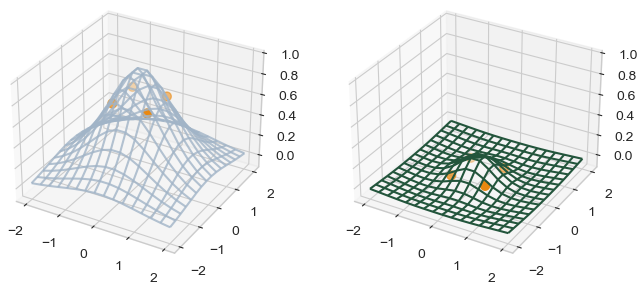
\includegraphics[width=\textwidth]{kernel2d.png}
        \end{figure}
      \end{column}
    \end{columns}
  \end{tcolorbox}

  \begin{tcolorbox}
    \blocktitle{\( k \)-th nearest neighbors?}

    \begin{columns}
      \begin{column}{0.5\textwidth}
        The screening effect suggests that one should simply
        pick the \( k \) closest points, recovering the \(
        k \)-th nearest neighbors (\( k \)-NN) algorithm.

        \vspace{\baselineskip}
        Here, the \textcolor{lightblue}{blue} points are the
        \textcolor{lightblue}{candidates}, the \textcolor{orange}{orange}
        point is the \textcolor{orange}{unknown} point, and the
        \textcolor{darkseagreen}{green} points are the \( k \)
        \textcolor{darkseagreen}{selected} points

        (in this example, \( k = 2 \)).
      \end{column}
      \begin{column}{0.5\textwidth}
        \begin{figure}[h!]
          \centering
          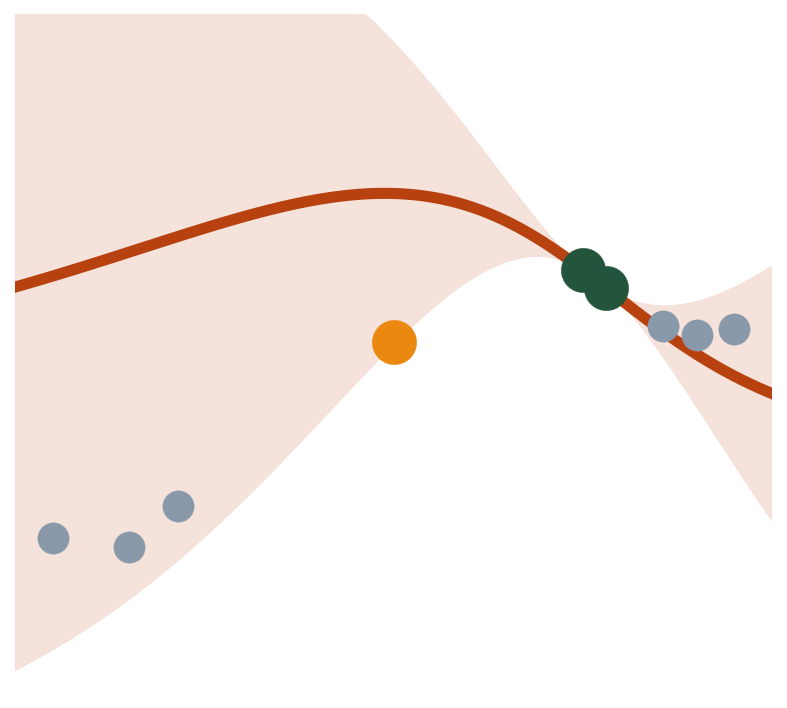
\includegraphics[width=\textwidth]{graphs/predict_knn_2.png}
        \end{figure}
      \end{column}
    \end{columns}
  \end{tcolorbox}

  \begin{tcolorbox}
    \blocktitle{\( k \)-NN is myopic, account for conditioning!}

    \textbf{Algorithm: [conditional \( k\)-th
      nearest neighbors (C\( k \)-NN)]:}

    \begin{columns}
      \begin{column}{0.5\textwidth}
        Selecting the closest point every iteration leads to redundancy.

        \vspace{\baselineskip}
        Instead, select points \emph{conditional} on points already selected.
        Selecting points by \emph{information} instead of by distance
        motivates conditional \( k \)-th nearest neighbors (C\( k \)-NN).
      \end{column}
      \begin{column}{0.5\textwidth}
        \begin{figure}[h!]
          \centering
          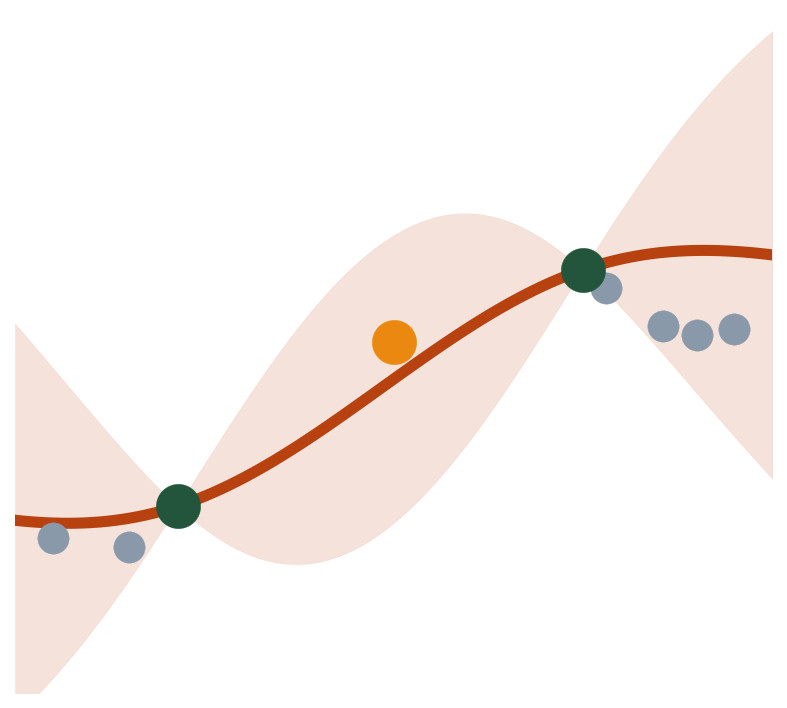
\includegraphics[width=\textwidth]{graphs/predict_cknn_2.png}
        \end{figure}
      \end{column}
    \end{columns}
  \end{tcolorbox}

  \begin{tcolorbox}
    \blocktitle{Greedy mutual information maximization}

    Greedily select the next training point with highest mutual
    information with the target point. If \( I \) is the set
    of selected indices, select by:
    \begin{align*}
      I &= I \cup
      \left \{
        \argmax_{j \not \in I} \:
          \frac{\Theta_{j, \text{Pr} \mid I}^2}{\Theta_{j, j \mid I}}
      \right \}
    \end{align*}
  \end{tcolorbox}
\end{column}

% https://tex.stackexchange.com/questions/504412/how-to-put-a-vertical-rule-between-beamer-columns-created-with-the-column-comma
% conveniently the rule doubles as a strut
\begin{column}{0.01\textwidth}
  \begin{center}
    \textcolor{darksilver}{\rule[-1cm]{1mm}{0.8\textheight}}
  \end{center}
\end{column}

%%% column 2

\begin{column}{0.30\textwidth}
  \begin{tcolorbox}
    \blocktitle{Efficient computation from Cholesky factor}

    A direct computation of the objective takes \(
    \mathcal{O}(N k^4) \) to select \( k \) points.

    This computational cost can be reduced to \( \mathcal{O}(N
    k^2) \) by storing a partial Cholesky factor, since
    each column is conditional on everything before it:
    \begin{align*}
      \chol(\Theta) &=
      \begin{pmatrix}
        I & 0 \\
        \textcolor{darkorange}{\Theta_{2, 1} \Theta_{1, 1}^{-1}} & I
      \end{pmatrix}
      \begin{pmatrix}
        \chol(\Theta_{1, 1}) & 0 \\
        0 & \chol(\textcolor{lightblue}{
          \Theta_{2, 2} - \Theta_{2, 1} \Theta_{1, 1}^{-1} \Theta_{1, 2}
        })
      \end{pmatrix}
    \end{align*}
  \end{tcolorbox}

  \begin{tcolorbox}
    \blocktitle{Generalization to multiple prediction points}

    For multiple prediction points, the objective becomes to minimize the
    log determinant of the conditional covariance matrix of prediction points.
    By making use of the matrix determinant lemma, one can show that:
    \begin{align*}
      \logdet
      \left (
        \Theta_{\text{Pr}, \text{Pr} \mid I \cup \{ k \}}
      \right ) -
      \logdet \left ( \Theta_{\text{Pr}, \text{Pr} \mid I} \right ) &=
      \log
      \left (
        \frac{\Theta_{kk \mid I, \text{Pr}}}{\Theta_{kk \mid I}}
      \right )
    \end{align*}
    We can efficiently compute the objective by storing \emph{two}
    Cholesky factors, yielding a complexity of \( \mathcal{O}(N
    k^2 + N m^2 + m^3) \) for \( m \) prediction points.
  \end{tcolorbox}

  \begin{tcolorbox}
    \blocktitle{Global approximation by KL-minimization}

    Approximate a Gaussian process by a sparse approximate Cholesky factor
    of its precision. Measure the resulting approximation accuracy by
    the KL divergence between the corresponding centered Gaussian processes:
    \begin{align*}
      L \coloneqq \argmin_{\hat{L} \in S} \, \mathbb{D}_{\text{KL}}
        \left (
          \mathcal{N}(\vec{0}, \Theta) \, \Big \| \,
          \mathcal{N}(\vec{0}, (\hat{L} \hat{L}^{\top})^{-1})
        \right )
    \end{align*}

    Using the optimal unique minimizer \( L \) from closed form computation:
    \begin{align*}
      L_{s_i, i} = \frac{\Theta_{s_i, s_i}^{-1} \vec{e}_1}
      {\sqrt{\vec{e}_1^{\top} \Theta_{s_i, s_i}^{-1} \vec{e}_1}}
    \end{align*}

    Objective becomes minimize variance of \(
    i \)th point, conditional on selected!
    \begin{align*}
      2 \mathbb{D}_{\text{KL}}
      \left (
        \mathcal{N}(\vec{0}, \Theta) \, \Big \| \,
        \mathcal{N}(\vec{0}, (L L^{\top})^{-1})
      \right )
      &= \sum_{i = 1}^N
        \left [
          \log \left ( \Theta_{ii \mid s_i - \{ i \}} \right )
        \right ]
        - \logdet(\Theta)
    \end{align*}
    % Sparsity of column of Cholesky factor \( \iff \) sparsity in selection
  \end{tcolorbox}

  \begin{tcolorbox}
    \blocktitle{Applying selection to Cholesky factorization}

    \begin{columns}
      \begin{column}{0.5\textwidth}
        For a column in isolation, \textcolor{orange}{unknown} point is the
        diagonal entry, below it are \textcolor{lightblue}{candidates}, and
        add \textcolor{seagreen}{selected} entries to the sparsity pattern
        \( s_i \).

        \vspace{\baselineskip}
        However, for multiple aggregated columns (supernodes), a candidate can
        be added ``partially'' if it is between prediction points. By careful
        application of rank-one downdating, this structure can be preserved at
        no additional cost.
      \end{column}
      \begin{column}{0.5\textwidth}
        \begin{figure}[h!]
          \centering
          \begin{tikzpicture}[scale=1]
            % outer triangular factor
\fill[lightsilver] (0, 0) -- (0, -16) -- (16, -16) -- cycle;

% column rectangle
\draw[fill=lightblue] (3, -4) rectangle (4, -16);

% triangular factor
\fill[silver] (0, 0) rectangle (1, -1);
\fill[silver] (1, -1) rectangle (2, -2);
\fill[silver] (1, -2) rectangle (2, -3);
\fill[silver] (2, -2) rectangle (3, -3);
\fill[orange] (3, -3) rectangle (4, -4);
\draw (3, -3) rectangle (4, -4);
\fill[silver] (0, -4) rectangle (1, -5);
\draw (3, -4) rectangle (4, -5);
\fill[silver] (4, -4) rectangle (5, -5);
\fill[silver] (1, -5) rectangle (2, -6);
\draw (3, -5) rectangle (4, -6);
\fill[silver] (5, -5) rectangle (6, -6);
\fill[silver] (2, -6) rectangle (3, -7);
\fill[seagreen] (3, -6) rectangle (4, -7);
\draw (3, -6) rectangle (4, -7);
\fill[silver] (4, -6) rectangle (5, -7);
\fill[silver] (6, -6) rectangle (7, -7);
\draw (3, -7) rectangle (4, -8);
\fill[silver] (7, -7) rectangle (8, -8);
\fill[silver] (0, -8) rectangle (1, -9);
\fill[silver] (2, -8) rectangle (3, -9);
\draw (3, -8) rectangle (4, -9);
\fill[silver] (4, -8) rectangle (5, -9);
\fill[silver] (8, -8) rectangle (9, -9);
\draw (3, -9) rectangle (4, -10);
\fill[silver] (6, -9) rectangle (7, -10);
\fill[silver] (7, -9) rectangle (8, -10);
\fill[silver] (8, -9) rectangle (9, -10);
\fill[silver] (9, -9) rectangle (10, -10);
\fill[silver] (2, -10) rectangle (3, -11);
\draw (3, -10) rectangle (4, -11);
\fill[silver] (5, -10) rectangle (6, -11);
\fill[silver] (6, -10) rectangle (7, -11);
\fill[silver] (8, -10) rectangle (9, -11);
\fill[orange] (10, -10) rectangle (11, -11);
\draw (3, -11) rectangle (4, -12);
\fill[silver] (7, -11) rectangle (8, -12);
\fill[silver] (8, -11) rectangle (9, -12);
\fill[silver] (10, -11) rectangle (11, -12);
\fill[silver] (11, -11) rectangle (12, -12);
\fill[silver] (0, -12) rectangle (1, -13);
\fill[seagreen] (3, -12) rectangle (4, -13);
\draw (3, -12) rectangle (4, -13);
\fill[silver] (4, -12) rectangle (5, -13);
\fill[silver] (6, -12) rectangle (7, -13);
\fill[seagreen] (10, -12) rectangle (11, -13);
\fill[silver] (11, -12) rectangle (12, -13);
\fill[silver] (12, -12) rectangle (13, -13);
\fill[seagreen] (3, -13) rectangle (4, -14);
\draw (3, -13) rectangle (4, -14);
\fill[silver] (7, -13) rectangle (8, -14);
\fill[silver] (9, -13) rectangle (10, -14);
\fill[silver] (12, -13) rectangle (13, -14);
\fill[orange] (13, -13) rectangle (14, -14);
\draw (3, -14) rectangle (4, -15);
\fill[silver] (5, -14) rectangle (6, -15);
\fill[silver] (9, -14) rectangle (10, -15);
\fill[silver] (10, -14) rectangle (11, -15);
\fill[silver] (11, -14) rectangle (12, -15);
\fill[silver] (12, -14) rectangle (13, -15);
\fill[silver] (13, -14) rectangle (14, -15);
\fill[silver] (14, -14) rectangle (15, -15);
\fill[silver] (1, -15) rectangle (2, -16);
\draw (3, -15) rectangle (4, -16);
\fill[silver] (5, -15) rectangle (6, -16);
\fill[silver] (9, -15) rectangle (10, -16);
\fill[silver] (11, -15) rectangle (12, -16);
\fill[silver] (12, -15) rectangle (13, -16);
\fill[silver] (13, -15) rectangle (14, -16);
\fill[silver] (14, -15) rectangle (15, -16);
\fill[silver] (15, -15) rectangle (16, -16);

% column rectangle
\draw (3, -4) rectangle (4, -16);

            \node[] at (12, -3) {
              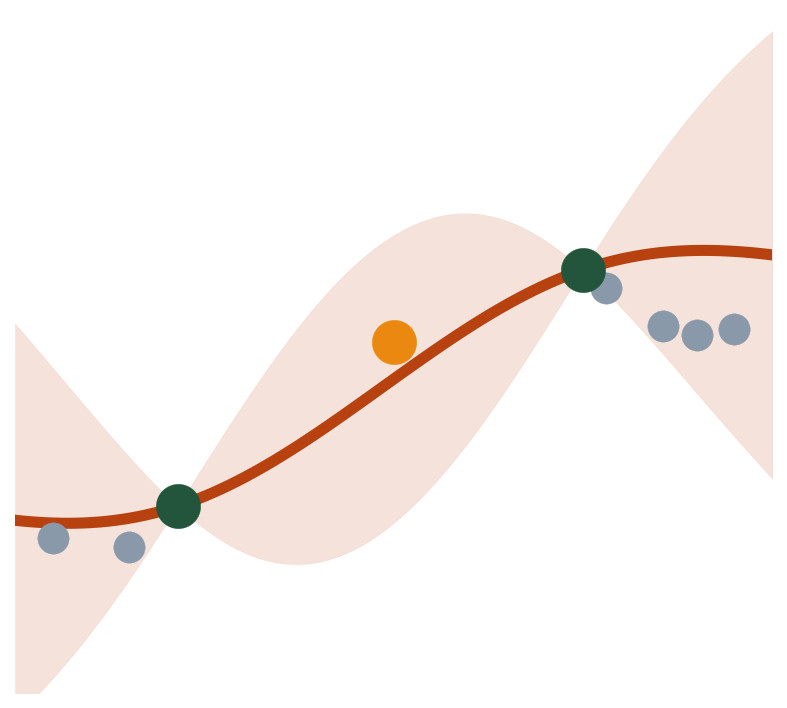
\includegraphics[width=0.5\textwidth]{graphs/predict_cknn_2}
            };
          \end{tikzpicture}
        \end{figure}
      \end{column}
    \end{columns}
  \end{tcolorbox}
\end{column}

\begin{column}{0.01\textwidth}
  \begin{center}
    \textcolor{darksilver}{\rule[-1cm]{1mm}{0.8\textheight}}
  \end{center}
\end{column}

%%% column 3

\begin{column}{0.30\textwidth}
  \begin{tcolorbox}
    \blocktitle{Drop-in replacement for \( k \)-NN on MNIST}

    \begin{columns}
      \begin{column}{0.5\textwidth}
        We classify an image by taking the mode label in \( k \)
        selected images. C\( k \)-NN gives better accuracies
        on the MNIST dataset for every \( k > 2 \).
      \end{column}
      \begin{column}{0.5\textwidth}
        \begin{figure}[h!]
          \centering
          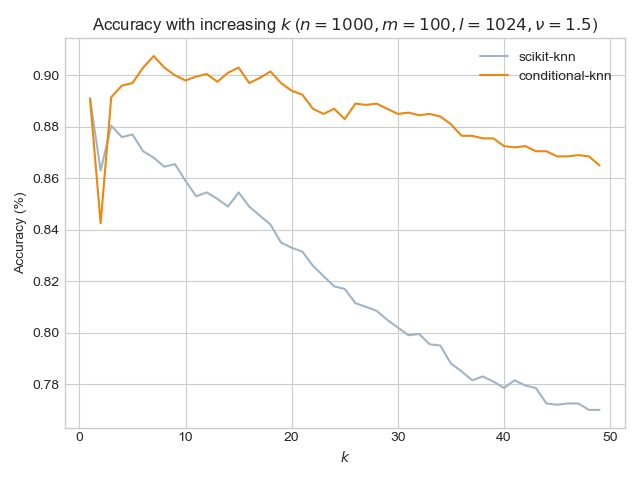
\includegraphics[width=\textwidth]{data/k_acc}
        \end{figure}
      \end{column}
    \end{columns}
  \end{tcolorbox}

  \begin{tcolorbox}
    \blocktitle{Recovery of sparse factors}

    \begin{columns}
      \begin{column}{0.5\textwidth}
        We generate random sparse Cholesky factors by randomly
        selecting a prescribed number of nonzero entries per column.

        C\( k \)-NN is able to recover the underlying sparse
        factor given its covariance with high accuracy.
      \end{column}
      \begin{column}{0.5\textwidth}
        \begin{figure}[h!]
          \centering
          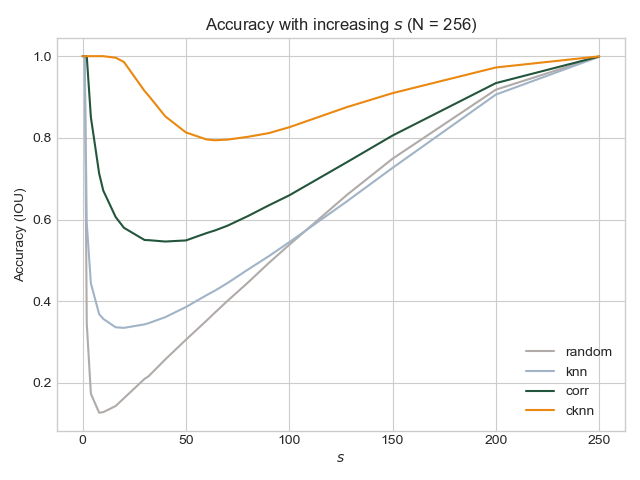
\includegraphics[width=\textwidth]{data/s_score.png}
        \end{figure}
      \end{column}
    \end{columns}
  \end{tcolorbox}

  \begin{tcolorbox}
    \blocktitle{Better KL divergence with sparser factors}

    \begin{columns}
      \begin{column}{0.5\textwidth}
        Plugging the selection algorithm into Cholesky
        factorization leads to better KL divergence for
        the same number of nonzero entries as \( k \)-NN.
      \end{column}
      \begin{column}{0.5\textwidth}
        \begin{figure}[h!]
          \centering
          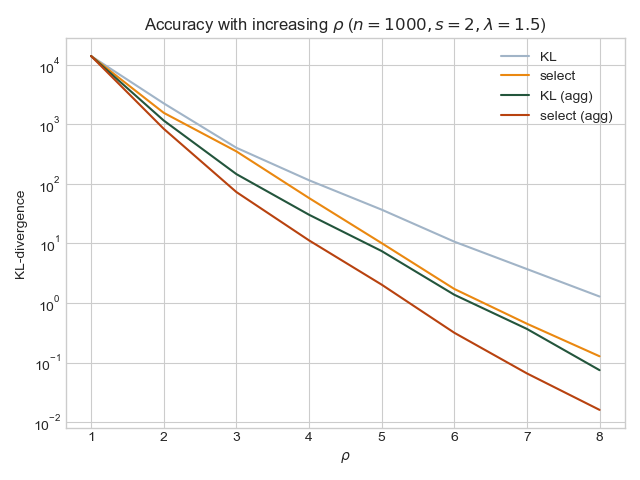
\includegraphics[width=\textwidth]{data/rho_kl-div.png}
        \end{figure}
      \end{column}
    \end{columns}
  \end{tcolorbox}

  \begin{tcolorbox}
    \blocktitle{Preconditioning with conjugate gradient}

    \begin{columns}
      \begin{column}{0.5\textwidth}
        Because the KL divergence strongly penalizes zero eigenvalues of the
        preconditioned matrix \( L \Theta L^T \), the condition number is
        improved, resulting in less iterations with the conjugate gradient.
      \end{column}
      \begin{column}{0.5\textwidth}
        \begin{figure}[h!]
          \centering
          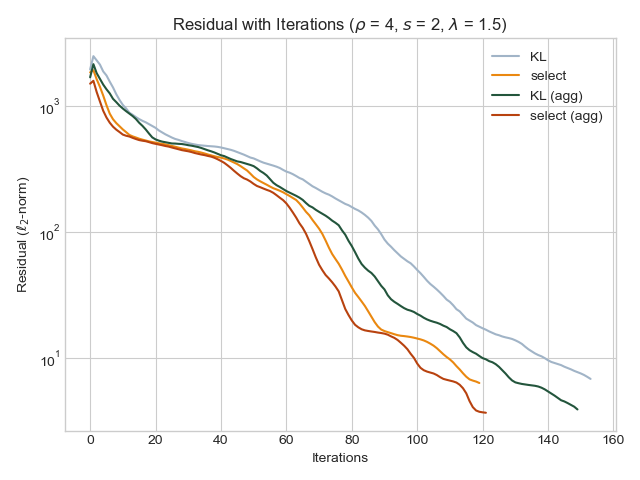
\includegraphics[width=\textwidth]{data/n_iter-res.png}
        \end{figure}
      \end{column}
    \end{columns}
  \end{tcolorbox}

\end{column}

\end{columns}

% \printbibliography

\end{frame}
\end{document}
